Ce livre a pour objectif de vous permettre de comprendre, décrire et quantifier le fonctionnement des machines thermodynamiques, c’est-à-dire les réfrigérateurs, les pompes à chaleur, et surtout les moteurs. Il est conçu pour être abordable en première année d’études supérieures et couvert en deux semestres environ. Il est destiné à de futur/es ingénieur/es curieux/ses de comprendre le pourquoi et le comment des machines qui les entourent et des équations qu’ils ou elles utilisent.

Il y a dix chapitres dans ce livre. Le \coursun recense les notions indispensables à notre étude.

Le chapitre le plus important est le \courssix~: c’est là que nous apprenons à transformer de la chaleur en travail et réciproquement. Cependant, pour pouvoir appliquer les concepts de ce chapitre à des cas concrets —par exemple pour pouvoir prédire par le calcul l’efficacité d’un moteur— nous avons besoin de plusieurs outils, auxquels sont consacrés les chapitres qui précèdent. Il nous faut d’abord disposer d’une méthode robuste de comptabilité de l’énergie : dans le \coursdeux nous comptabilisons les transferts dans une quantité fixe de fluide, et dans le \courstrois nous comptabilisons ces transferts dans un fluide en flux continu. Il nous faut également savoir prédire la température et quantifier l’énergie dans les fluides utilisés en pratique, ce que nous faisons pour l’air dans le \coursquatre et pour l’eau dans le \courscinq. Ainsi, à la fin du \courssixshort, vous saurez quantifier la transformation de chaleur et de travail au sein de tous types de machines.

Une particularité des machines thermodynamiques est qu’elles sont toutes très inefficaces. L’exploration des causes de ces inefficacités et la quantification de leurs limites théoriques font l’objet du \courssept. Cette exploration culmine avec le \courshuitshort où nous apprenons à nous servir de l’\textit{entropie}, un extraordinaire et puissant concept physique, pour décrire les transformations dans nos machines.

Avec ces notions, vous serez à même de comprendre et quantifier le fonctionnement de deux grands types de moteurs utilisés dans l’industrie : les centrales à vapeur, décrites dans le \coursneuf, et les moteurs à combustion interne, décrits dans le \coursdix.

\onlyamphibook{\clearpage\thispagestyle{empty}}%handmade
\begin{center}
	\onlyframabook{\vspace{1cm}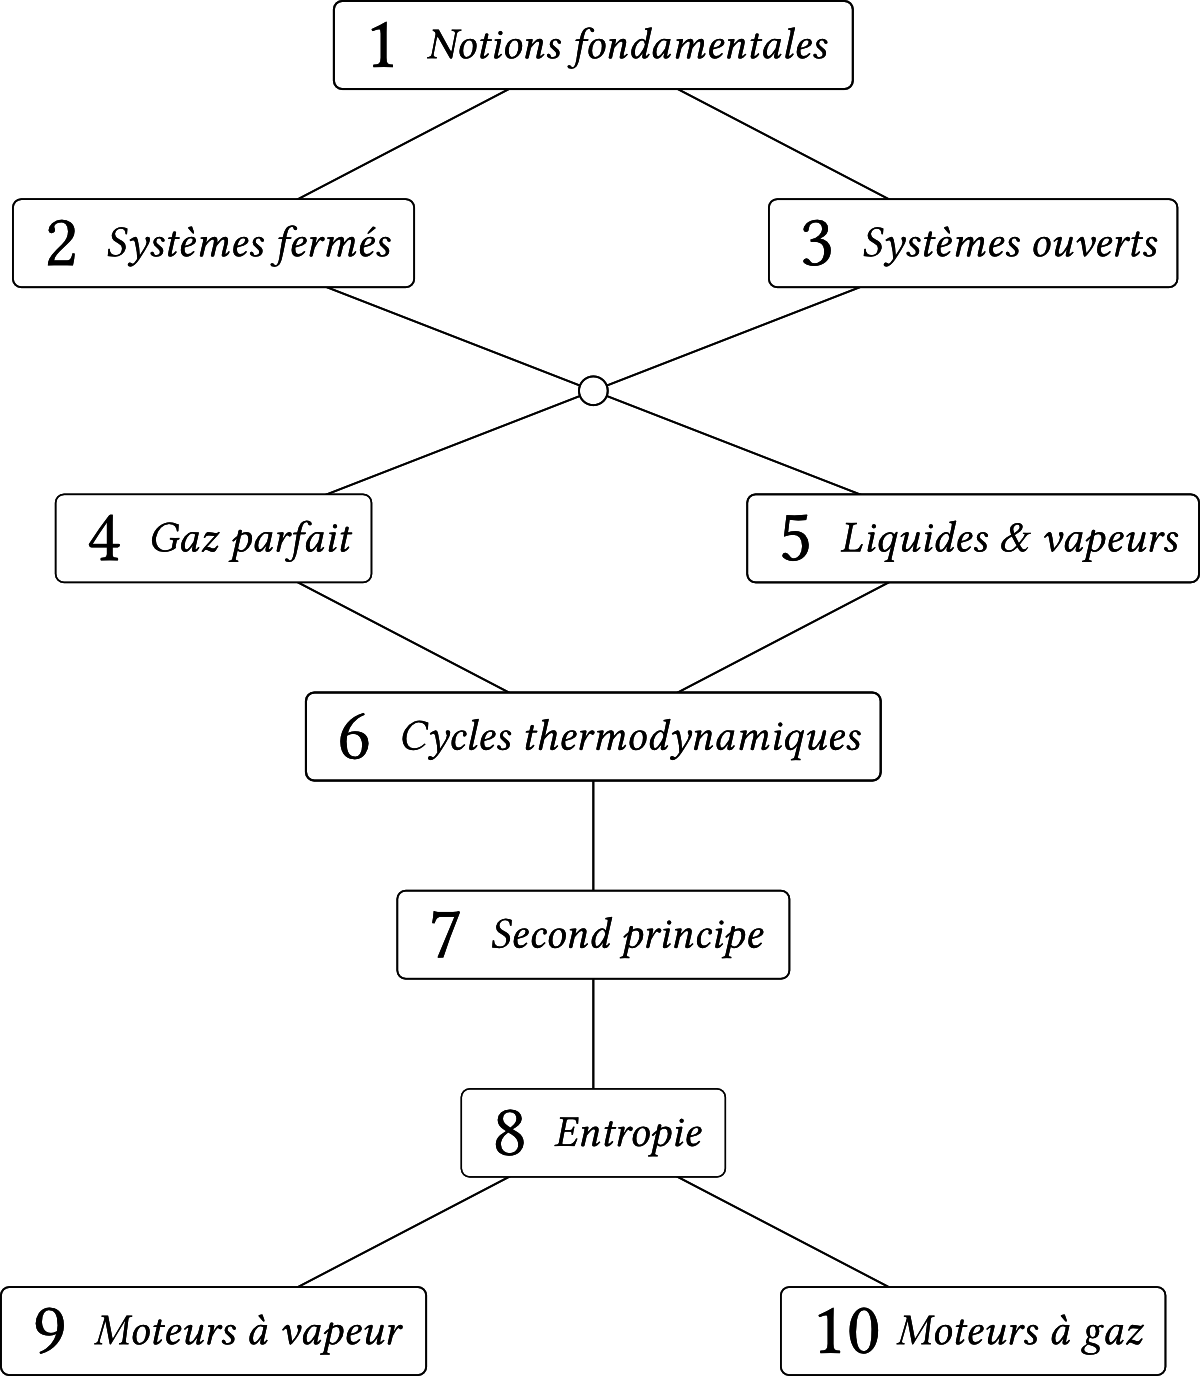
\includegraphics[width=0.7\textwidth]{images/plan_general_chapitres.png}\vspace{1cm}}%handmade
	\onlyamphibook{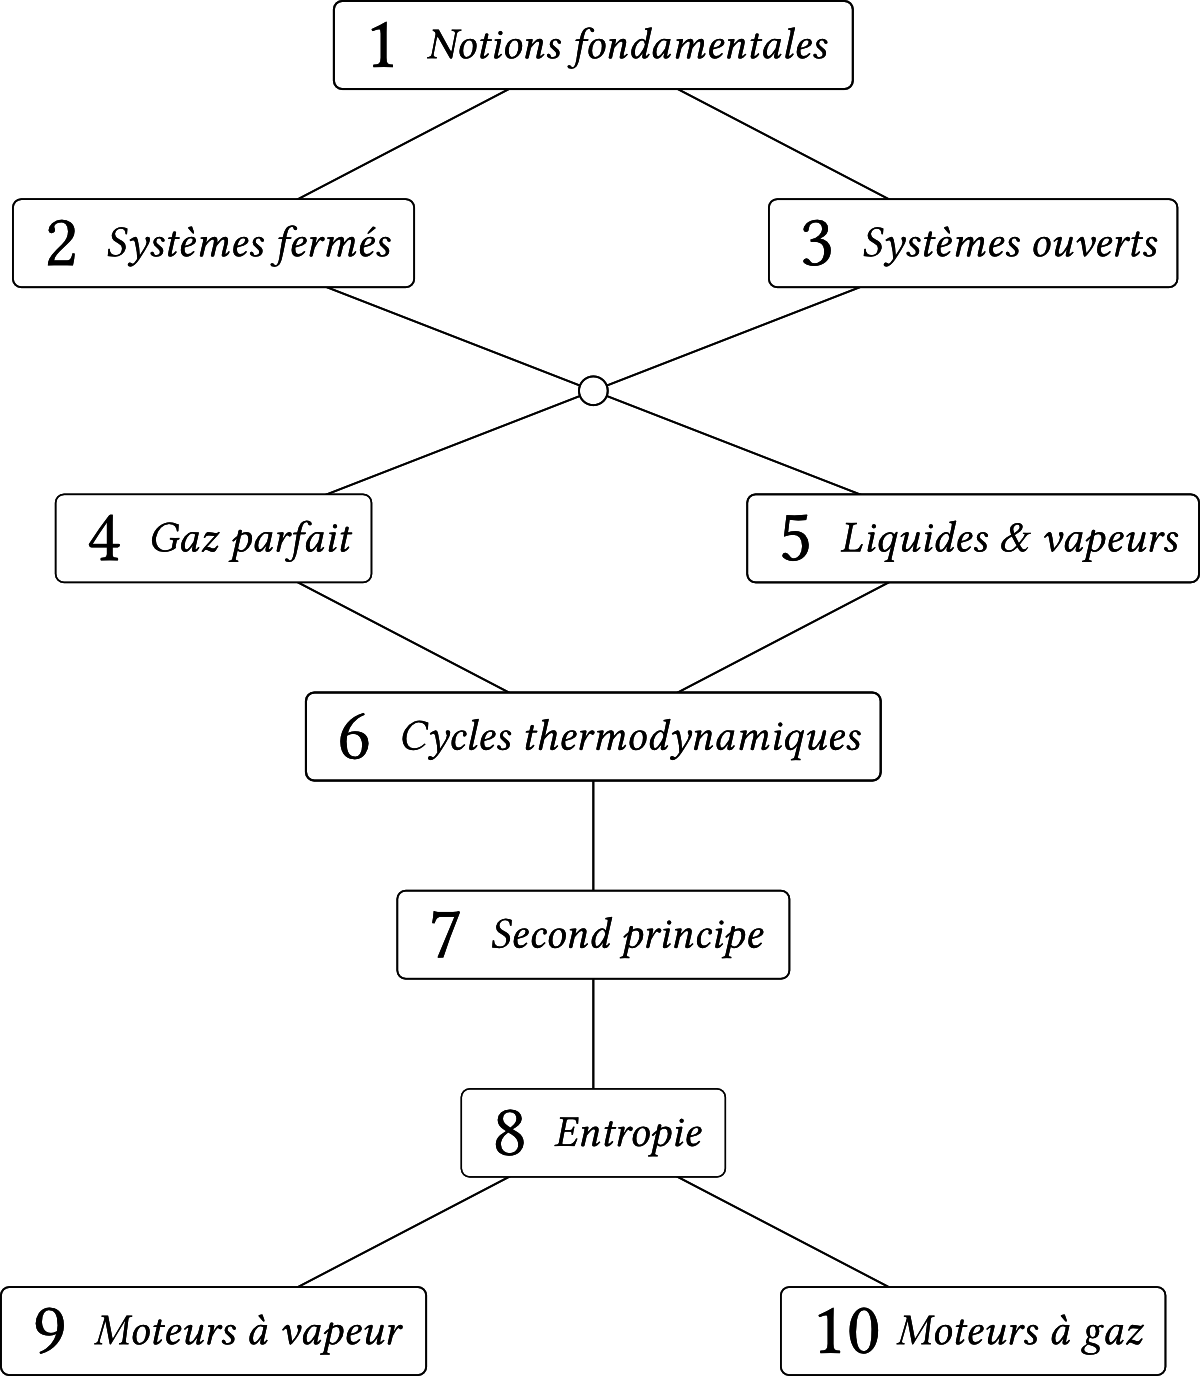
\includegraphics[width=0.65\textwidth]{images/plan_general_chapitres.png}}
\end{center}

À la fin de chaque chapitre, une série de problèmes concrets est présentée. Ces exercices sont là pour votre entraînement, mais aussi pour votre motivation : ils présentent le type de problème que nous cherchons à résoudre avec le chapitre. Afin de vous permettre de vous former seul/e, la solution de chaque exercice est brièvement décrite en dernière page. Je vous conseille de ne jamais y avoir recours avant d’avoir transpiré au moins une heure, car une fois que l’on a lu la méthode de résolution, il est impossible de faire comme si l’on ne la connaissait pas !

Vous trouverez aussi à la fin de chaque chapitre une courte section historique. Ces petits éléments de contexte nous ont semblé, à moi-même et Philippe Depondt, pouvoir contribuer à votre culture de scientifique et d’ingénieur/e. 

Enfin, le livre que vous avez entre les mains est véritablement \emph{à vous} : il est publié sous une licence libre dont les termes sont détaillés en annexe~\ref{ch_remix}. Il me paraît en effet important que vous puissiez non seulement le partager librement et gratuitement (en le photocopiant, en en faisant des copies numériques, etc.) mais aussi le remixant d’une façon ou d’une autre (en l’améliorant, le raccourcissant ou l’adaptant à d’autres formes par exemple) en fonction de vos besoins, vous appropriant ainsi véritablement son contenu.

Mon espoir est qu’après avoir utilisé ce livre, le son d’une turbomachine en fonctionnement ne puisse vous laisser ni perplexe ni insensible. Bon courage !

\begin{flushright}Olivier Cleynen\\ \textit{février 2015}\end{flushright}
